\begin{minipage}{\linewidth}  % Minipage with full line width
    \vspace{1cm}
        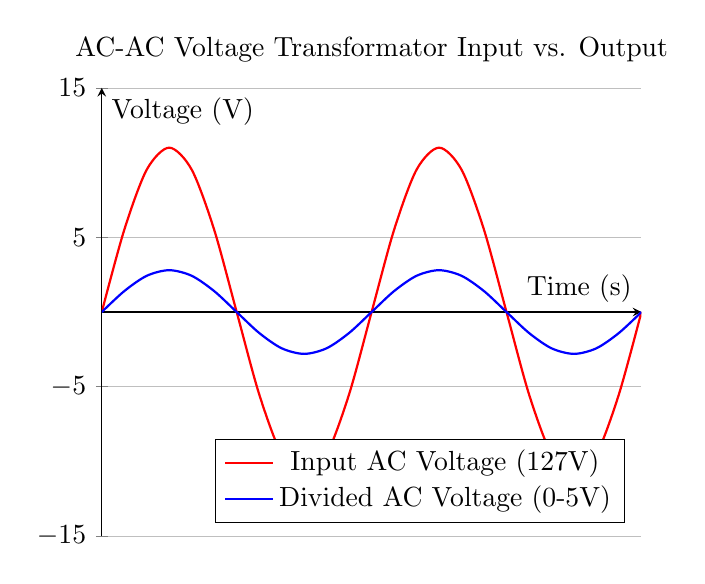
\begin{tikzpicture}
            \begin{axis}[
                title={AC-AC Voltage Transformator Input vs. Output},
                %width=0.8\linewidth,  % Adjust width to be the full line width
                %height=\linewidth,  % Adjust height to fit better
                xlabel={Time (s)},
                ylabel={Voltage (V)},
                xmin=0, xmax=2*pi,
                ymin=-15, ymax=15,
                xtick=\empty,
                ytick={-15, -5, 0, 5, 15},
                axis x line=middle,
                axis y line=middle,
                legend pos=south east,
                grid=both,
                major grid style={line width=.2pt,draw=gray!50},
                minor grid style={line width=.1pt,draw=gray!20},
                domain=0:2*pi,
            ]

            % Plot the 127V input signal (scaled for illustration)
            \addplot[smooth, thick, red] {11 * sin(deg(2*x))};
            \addlegendentry{Input AC Voltage (127V)}

            % Plot the divided signal, scaled to 0-5V for Arduino
            \addplot[smooth, thick, blue] {2.8 * sin(deg(2*x))};
            \addlegendentry{Divided AC Voltage (0-5V)}

            \label{fig:voltage-divider-graph}
            \end{axis}
        \end{tikzpicture}
\end{minipage}
\vspace{2pt}
